\chapter{Application Detection}
Similar to website fingerprinting, we try to identify the application running on target note by its traffic. This chapter discusses some general idea without a specific application.

\section{Network Protocol Headers}
Since most information in MAC\footnote{Media Access Control, not to be confused with the cryptographic term Message Authenticate Code.}, IP and UDP headers are related to routing and network maintenance and thus independent except the length fields and CRC\footnote{Cyclic Redundancy Check, a code to detect or correct transmission error}. 

\section{Packet Length}
Packet length is usually the most interested target in traffic analysis. However, packet lengths are also highly application dependant; thus we are not pursuing this topic further without a specific application.

\section{Timing Packet Response}
Unlike web applications where the client and server are usually physically distant, sensor networks can sometimes located in a concentrated area, such as a house which its radius can be less than 10 meters. 

These features theoretically enables one to capture all traffics in such a sensor network. As opposed to the case of Internet where packets are usually timed on the client’s side and thus network latency (RTT\footnote{Round-Trip Time}) must be concerned, being able to capture all traffic in the network provides  much more accurate timing information and hence may be exploited to develop more efficient attacks.

\begin{definition}
In a Request-Response application model, \textbf{RI}, {\bf Response Interval}, is defined as the interval between a request packet being received and its response being sent.
\end{definition}

\begin{example}
\begin{figure}
\centering
{
	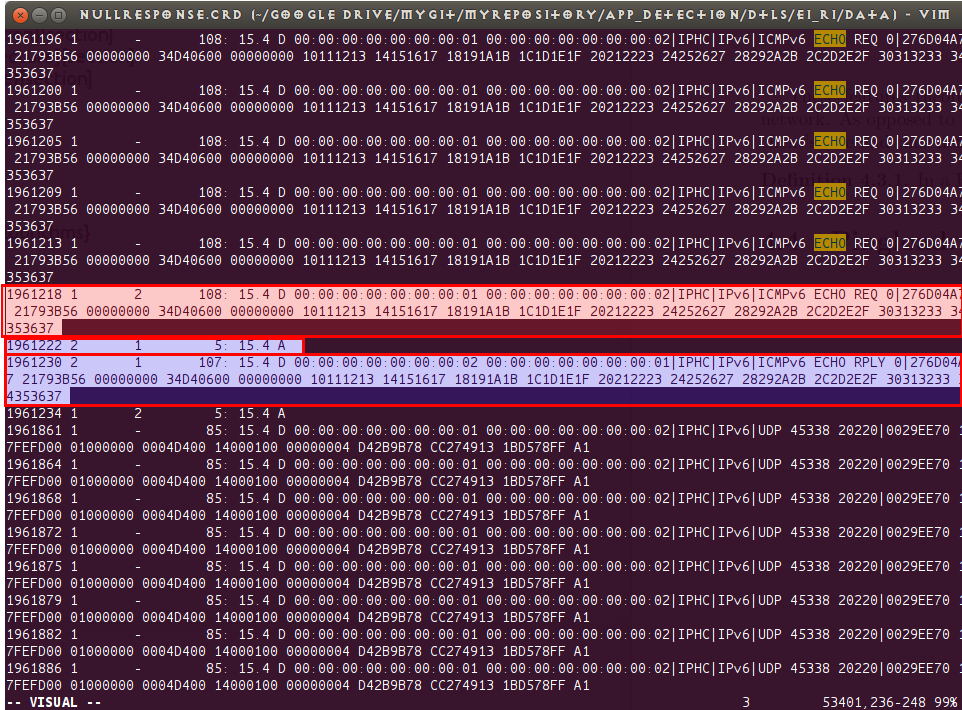
\includegraphics[width=\textwidth,]{fig/responsetime.png}
}
\caption{Capture of a ping packet}
\label{fig: ping packet}
\end{figure}

\begin{table}[!]
\centering
\begin{tabular}{|l|l|l|l|l|}
\hline
Time (ms) & From (ID) & To (ID) & Length (bytes) & Type          \\ \hline
1961218   & 1         & 2       & 108            & ICMP ECHO \\ \hline
1961222   & 2         & 1       & 5              & 802.15.4 ACK  \\ \hline
1961230   & 2         & 1       & 107            & ICMP ECHO \\ \hline
\end{tabular}
\caption{Packet Features of an ICMP ECHO request and response}
\label{Tbl: ping}
\end{table}

Three packets are marked out in \Cref{fig: ping packet} which forms an instance of ICMP ECHO\cite{rfc1122} (also known as PING) session. The extracted packet features are displayed in \Cref{Tbl: ping}.

\begin{description}
\item[Explanation of the Packets:]\hfill \\
The first packet is an ICMP ECHO request and the third packet being its response. The second packet is a 802.15.4 ACK\footnote{This is an acknowledgement from the receiver that notifies the sender that the packet has been received.} and is thus transparent to the upper ICMP protocol.
\end{description}

From this example we can see that the RI for this PING session is:
\begin{equation*}
1961230 - 1961218 = 12 \text{(ms)}
\end{equation*}

\end{example}

Timing information can be exploited by several attacks, such as \cite{Peekaboo} and \cite{rsatiming}.

We have experimentally measured a RNG\footnote{Random Number Generator} call on Wismote platform in the Cooja simulator is roughly 0.3 ms.

\section{PINGLOAD: PING side-channel for Payload }
Support of ICMP ECHO is required by \cite{rfc1122} and is also enabled in Contiki OS by default. However, our experimental results shows that the response time of these ping packets could potentially be exploited to reveal the application running on target sensor node.

We call such technique {\bf  Application Fingerprinting}.

\subsection{Hypothesis}
A phenomenon we realised is that when a ping packet arrived while the target node is executing some payload, say reading a sensor or processing data, the PING RI begins to vary comparing to a stable value  when no there is no payload. 

\begin{example}
\begin{figure}
\centering
{
  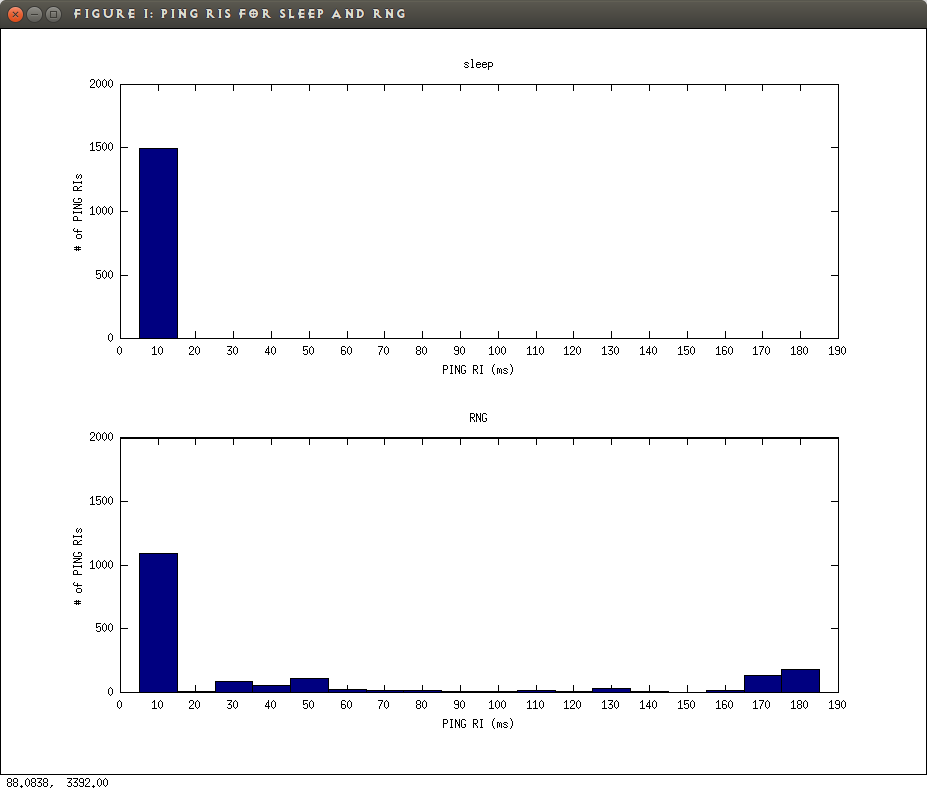
\includegraphics[width=0.9\textwidth]{fig/pingri.png}
}
\caption{An example of PING’s RIs with different payload}
\label{Fig: PINGLOAD RIs}
\end{figure}
\Cref{Fig: PINGLOAD RIs} shows RIs of PING collected in two experiments. The left half are collected with the target is constantly idle whilst the right half occasionally receives a request which triggers the target to call RNG. We can see that the PING RI varies alongside the target is given some payload.
\end{example}

The data shown in \Cref{Fig: PINGLOAD RIs} suggests that the “plain”, that is without any interference, PING RI is 12 to 13 ms. Further more, those variations of  PING RI is very likely caused by the payload of the target.

This experiment inspirits that the distributions of PING RIs might vary according to the payload of target and could possibly considered as an fingerprint of the target’s application. In other word, an adversary could possibly tell whether the target is running a specific application by looking at its PING RIs distribution.

DESCRIBE HOW TO DO THE ATTACK HERE

\subsection{Experiment Result}

\subsection{General Hypothetical Model}